\documentclass{article}
\usepackage{import}
\import{../../../lib/latex/}{wgmlgz}


\begin{document}

\itmo[
  variant=19489,
  labn=4,
  discipline=Основы профессиональной деятельности,
  group=P3115,
  student=Владимир Мацюк,
  teacher=Абузов Ярослав Александрович,
  logo=../../../lib/img/itmo.png
]

\section{Текст задания}
По выданному преподавателем варианту восстановить текст заданного варианта программы, определить предназначение и составить описание программы, определить область представления и область допустимых значений исходных данных и результата, выполнить трассировку программы.
\begin{center}
  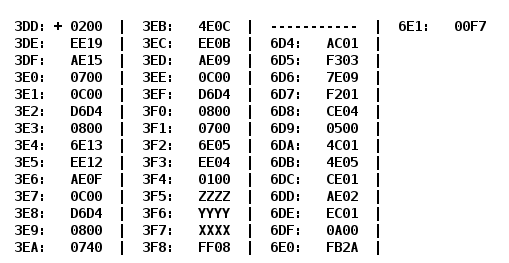
\includegraphics[scale=0.8]{task.png}
\end{center}
\begin{tabular}{|c|r|l|l|} \hline
  Адрес & Код команды & Мнемоника         & Комментарии \nl
  3DD   & +0200       & CLA               & Очистка аккумулятора \nl
  3DE   & EE19        & ST IP+19  (r)     & Сохранение (Прямая относительная адресация) \nl
  3DF   & AE15        & LD IP+15  (z)     & Загрузка (Прямая относительная адресация) \nl
  3E0   & 0700        & INC               & Инкремент \nl
  3E1   & 0C00        & PUSH              & Запись в стэк \nl
  3E2   & D6D4        & CALL 0x6D4        & Вызов подпрограммы (Прямая абсолютная адресация) \nl
  3E3   & 0800        & POP               & Чтение из стэка \nl

  3E4   & 6E13        & SUB IP+13 (r)     & Вычитание (Прямая относительная адресация) \nl
  3E5   & EE12        & ST IP+12 (r)      & Сохранение (Прямая относительная адресация) \nl
  3E6   & AE0F        & LD IP+F  (y)      & Загрузка (Прямая относительная адресация) \nl
  3E7   & 0C00        & PUSH              & Запись в стэк \nl
  3E8   & D6D4        & CALL 0x6D4        & Вызов подпрограммы (Прямая абсолютная адресация) \nl
  3E9   & 0800        & POP               & Чтение из стэка \nl

  3EA   & 0740        & DEC               & Декремент \nl
  3EB   & 4E0C        & ADD IP+C (r)      & Сложение (Прямая относительная адресация) \nl
  3EC   & EE0B        & ST IP+B  (r)      & Сохранение (Прямая относительная адресация) \nl
  3ED   & AE09        & LD IP+9 (x)       & Загрузка (Прямая относительная адресация) \nl
  3EE   & 0C00        & PUSH              & Запись в стэк \nl
  3EF   & D6D4        & CALL 0x6D4        & Вызов подпрограммы (Прямая абсолютная адресация) \nl
  3F0   & 0800        & POP               & Чтение из стэка \nl

  3F1   & 0700        & INC               & Инкремент \nl
  3F2   & 6E05        & SUB IP+5 (r)      & Вычитание (Прямая относительная адресация) \nl
  3F3   & EE04        & ST IP+4  (r)      & Сохранение (Прямая относительная адресация) \nl
  3F4   & 0100        & HLT               & Остановка \nl

  3F5   & ZZZZ        & Переменная/ошибка & z \nl
  3F6   & YYYY        & Переменная/ошибка & y \nl
  3F7   & XXXX        & Переменная/ошибка & x \nl
  3F8   & FF08        & Константа/ошибка  & r \nl
  6D4   & AC01        & LD (SP+1)         & Загрузка (Косвенная относительная со смещением) \nl
  605   & F303        & BPL IP+3 (a)      & Переход, если плюс \nl
  6D6   & 7E09        & CMP IP+9 (A)      & Сравнение (Прямая относительная адресация) \nl
  6D7   & F201        & BMI IP+1 (a)      & Переход, если минус \nl
  6D8   & CE04        & BR IP+4 (b)       & Безусловный переход (эквивалент JUMP c прямой относительной адресацией) \nl
  6D9   & 0500        & a: ASL            & Арифметический сдвиг влево \nl
  6DA   & 4C01        & ADD (SP+1)        & Сложение (Косвенная относительная со смещением) \nl
  6DB   & 4E05        & ADD IP+5  (B)     & Сложение (Прямая относительная адресация) \nl
  6DC   & CE01        & BR IP+1 (c)       & Безусловный переход (эквивалент JUMP c прямой относительной адресацией) \nl
  6DD   & AE02        & b: LD IP+2  (A)   & Загрузка (Прямая относительная адресация) \nl
  6DE   & EC01        & c: ST (SP+1)      & Сохранение (Косвенная относительная со смещением) \nl
  6DF   & 0A00        & RET               & Возврат из подпрограммы \nl
  6E0   & FB2A        & A                 & \nl
  641   & 00F7        & B                 & \nl
\end{tabular}

\section{Описание программы}


Программа находит количесво отрицательных чисел и сохраняет результат в ячейке 4D3.
Псевдокод:


% asm


% \begin{lstlisting}

% ac = 0
% t = ac
% ac = z
% ++ac
% ac = f(ac)

% ac -= t
% t = ac
% ac = y
% ac = f(ac)

% --ac
% ac += t
% t = ac
% ac = x
% ac = f(ac)

% ++ac
% ac -= t

% \end{lstlisting}




% \begin{lstlisting}

%   ac = arg
%   if ac > 0: jpm a
%   cmp A
%   if ac < 0: jmp a

%   jmp b

%   a: ac <<= 1
%   ac += arg
%   ac += B
%   jmp c

%   b: ac = a

%   c: arg = ac
%   ret 


% \end{lstlisting}


% c


% \begin{lstlisting}

% ac = 0
% t = ac
% ac = z
% ++ac
% ac = f(ac)

% ac -= t
% t = ac
% ac = y
% ac = f(ac)

% --ac
% ac += t
% t = ac
% ac = x
% ac = f(ac)

% ++ac
% ac -= t
% t = ac


% \end{lstlisting}


% \begin{lstlisting}
% f(x)
%   ac = x
%   if ac >= 0 || ac < A
%     ac <<= 1
%     ac += x
%     ac += B
%   else
%     ac = a

%   return ac 
% \end{lstlisting}

% js


\begin{lstlisting}
t = 0
t = f(z + 1) - t
t = f(y) - 1 + t
t = f(x) + 1 - t
\end{lstlisting}
\begin{lstlisting}
f = (x) => (x >= 0 || x < A) ? 3x + B : A
\end{lstlisting}

$$
  f(x) = \begin{cases}
    3x + B,\  x \ge 0\ |\ x < A \\
    A
  \end{cases}
$$
$$   A = -1238,\ B = 247$$
$$    R = f(x) - f(y) - f(z + 1) + 2 $$
\begin{center}
  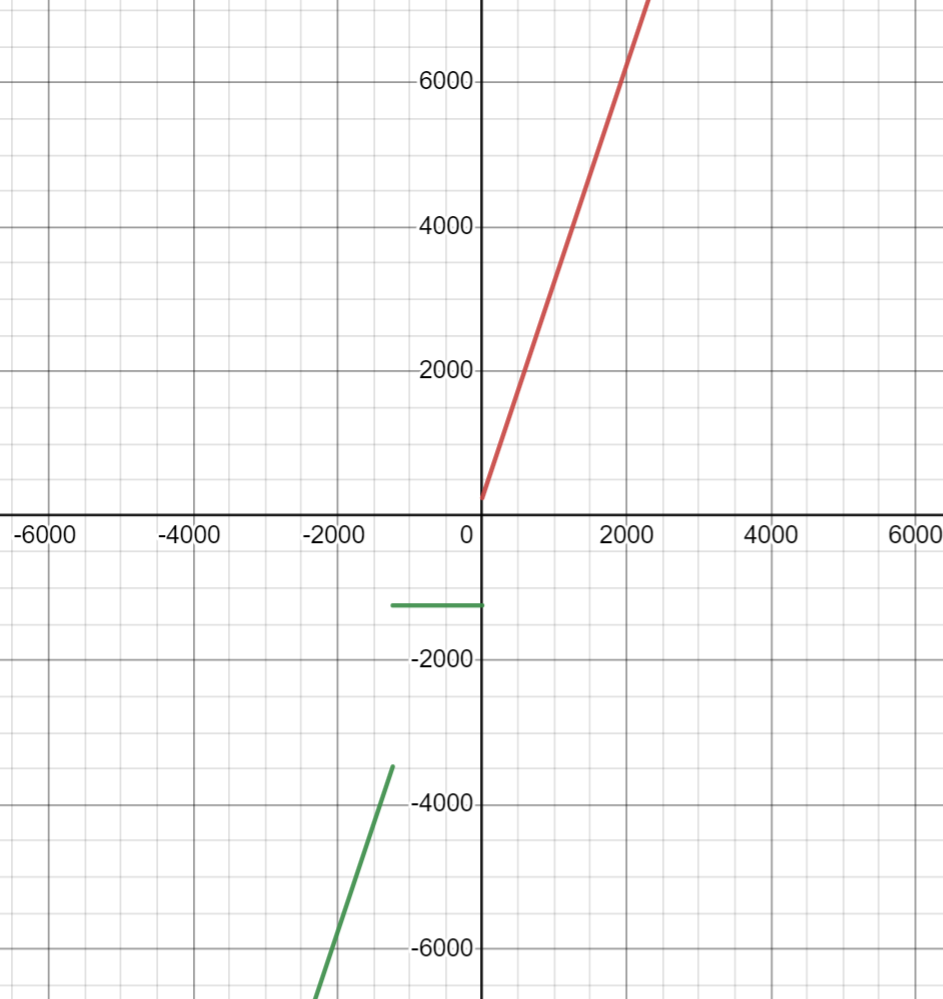
\includegraphics[scale=0.4]{graph.png}
\end{center}
\section{Область представления}
\begin{itemize}
  \item x, y, z, r, a, b - целые знаковые шестнадцатеричные числа в дополнительном коде
\end{itemize}

\section{Расположение данных в памяти}

\begin{itemize}
  \item Основная программа:
        \begin{itemize}
          \item 10C-126 – команды;
          \item 127, 128, 129 – исходные данные;
          \item 12A – итоговый результат.
        \end{itemize}
  \item Подпрограмма:
        \begin{itemize}
          \item 6ED-6F8 – команды;
          \item 6F9, 6FA – константы.
        \end{itemize}
\end{itemize}

\section{Адреса первой и последней выполняемой команды}

\begin{itemize}
  \item Основная программа:
        \begin{itemize}
          \item Адрес первой команды: 4D4
          \item Адрес последней команды: 4Df
        \end{itemize}
  \item Подпрограмма:
        \begin{itemize}
          \item Адрес первой команды: 4D4
          \item Адрес последней команды: 4Df
        \end{itemize}
\end{itemize}


\section{Таблица трассировки}

\begin{tabular}{|c|c|c|c|c|c|c|c|c|c|c|c|c|c|c|} \hline
  Адр & Код  & IP  & CR   & AR  & DR   & SP  & BR   & AC   & PS  & NZVC & Адр & Код \nl
  4D4 & 0200 & 4D4 & 0000 & 000 & 0000 & 000 & 0000 & 0000 & 004 & 0100 &     & \nl
  4D4 & 0200 & 4D5 & 0200 & 4D4 & 0200 & 000 & 04D4 & 0000 & 004 & 0100 &     & \nl
  4D5 & EEFD & 4D6 & EEFD & 4D3 & 0000 & 000 & FFFD & 0000 & 004 & 0100 & 4D3 & 0000 \nl
  4D6 & AF04 & 4D7 & AF04 & 4D6 & 0004 & 000 & 0004 & 0004 & 000 & 0000 &     & \nl
  4D7 & EEFA & 4D8 & EEFA & 4D2 & 0004 & 000 & FFFA & 0004 & 000 & 0000 & 4D2 & 0004 \nl
  4D8 & AEF7 & 4D9 & AEF7 & 4D0 & 04E0 & 000 & FFF7 & 04E0 & 000 & 0000 &     & \nl
  4D9 & EEF7 & 4DA & EEF7 & 4D1 & 04E0 & 000 & FFF7 & 04E0 & 000 & 0000 & 4D1 & 04E0 \nl

  4DA & AAF6 & 4DB & AAF6 & 4E0 & 44D4 & 000 & FFF6 & 44D4 & 000 & 0000 & 4D1 & 04E1 \nl
  4DB & F301 & 4DD & F301 & 4DB & F301 & 000 & 0001 & 44D4 & 000 & 0000 &     & \nl
  4DD & 84D2 & 4DE & 84D2 & 4D2 & 0003 & 000 & 0002 & 44D4 & 000 & 0000 & 4D2 & 0003 \nl
  4DE & CEFB & 4DA & CEFB & 4DE & 04DA & 000 & FFFB & 44D4 & 000 & 0000 &     & \nl

  4DA & AAF6 & 4DB & AAF6 & 4E1 & CE00 & 000 & FFF6 & CE00 & 008 & 1000 & 4D1 & 04E2 \nl
  4DB & F301 & 4DC & F301 & 4DB & F301 & 000 & 04DB & CE00 & 008 & 1000 &     & \nl
  4DC & 3AF6 & 4DD & 3AF6 & 000 & 0000 & 000 & 31FF & CE00 & 008 & 1000 & 4D3 & 0001 \nl
  4DD & 84D2 & 4DE & 84D2 & 4D2 & 0002 & 000 & 0001 & CE00 & 008 & 1000 & 4D2 & 0002 \nl
  4DE & CEFB & 4DA & CEFB & 4DE & 04DA & 000 & FFFB & CE00 & 008 & 1000 &     & \nl

  4DA & AAF6 & 4DB & AAF6 & 4E2 & 0900 & 000 & FFF6 & 0900 & 000 & 0000 & 4D1 & 04E3 \nl
  4DB & F301 & 4DD & F301 & 4DB & F301 & 000 & 0001 & 0900 & 000 & 0000 &     & \nl
  4DD & 84D2 & 4DE & 84D2 & 4D2 & 0001 & 000 & 0000 & 0900 & 000 & 0000 & 4D2 & 0001 \nl
  4DE & CEFB & 4DA & CEFB & 4DE & 04DA & 000 & FFFB & 0900 & 000 & 0000 &     & \nl

  4DA & AAF6 & 4DB & AAF6 & 4E3 & 0900 & 000 & FFF6 & 0900 & 000 & 0000 & 4D1 & 04E4 \nl
  4DB & F301 & 4DD & F301 & 4DB & F301 & 000 & 0001 & 0900 & 000 & 0000 &     & \nl
  4DD & 84D2 & 4DF & 84D2 & 4D2 & 0000 & 000 & FFFF & 0900 & 000 & 0000 & 4D2 & 0000 \nl
  4DF & 0100 & 4E0 & 0100 & 4DF & 0100 & 000 & 04DF & 0900 & 000 & 0000 &     & \nl
\end{tabular}

\section{Вывод}

Во время выполнения лабораторной работы я научился вызывать и исследовать подпрограммы, работать
со стеком, изучил цикл выполнения таких команд как CALL и RET.

\end{document}
